% Generated by Sphinx.
\def\sphinxdocclass{report}
\documentclass[letterpaper,10pt,english]{sphinxmanual}
\usepackage[utf8]{inputenc}
\DeclareUnicodeCharacter{00A0}{\nobreakspace}
\usepackage{cmap}
\usepackage[T1]{fontenc}
\usepackage{babel}
\usepackage{times}
\usepackage[Bjarne]{fncychap}
\usepackage{longtable}
\usepackage{sphinx}
\usepackage{multirow}


\title{ROSMOD Documentation}
\date{May 22, 2015}
\release{0.3}
\author{Pranav Srinivas Kumar}
\newcommand{\sphinxlogo}{}
\renewcommand{\releasename}{Release}
\makeindex

\makeatletter
\def\PYG@reset{\let\PYG@it=\relax \let\PYG@bf=\relax%
    \let\PYG@ul=\relax \let\PYG@tc=\relax%
    \let\PYG@bc=\relax \let\PYG@ff=\relax}
\def\PYG@tok#1{\csname PYG@tok@#1\endcsname}
\def\PYG@toks#1+{\ifx\relax#1\empty\else%
    \PYG@tok{#1}\expandafter\PYG@toks\fi}
\def\PYG@do#1{\PYG@bc{\PYG@tc{\PYG@ul{%
    \PYG@it{\PYG@bf{\PYG@ff{#1}}}}}}}
\def\PYG#1#2{\PYG@reset\PYG@toks#1+\relax+\PYG@do{#2}}

\expandafter\def\csname PYG@tok@gd\endcsname{\def\PYG@tc##1{\textcolor[rgb]{0.63,0.00,0.00}{##1}}}
\expandafter\def\csname PYG@tok@gu\endcsname{\let\PYG@bf=\textbf\def\PYG@tc##1{\textcolor[rgb]{0.50,0.00,0.50}{##1}}}
\expandafter\def\csname PYG@tok@gt\endcsname{\def\PYG@tc##1{\textcolor[rgb]{0.00,0.27,0.87}{##1}}}
\expandafter\def\csname PYG@tok@gs\endcsname{\let\PYG@bf=\textbf}
\expandafter\def\csname PYG@tok@gr\endcsname{\def\PYG@tc##1{\textcolor[rgb]{1.00,0.00,0.00}{##1}}}
\expandafter\def\csname PYG@tok@cm\endcsname{\let\PYG@it=\textit\def\PYG@tc##1{\textcolor[rgb]{0.25,0.50,0.56}{##1}}}
\expandafter\def\csname PYG@tok@vg\endcsname{\def\PYG@tc##1{\textcolor[rgb]{0.73,0.38,0.84}{##1}}}
\expandafter\def\csname PYG@tok@m\endcsname{\def\PYG@tc##1{\textcolor[rgb]{0.13,0.50,0.31}{##1}}}
\expandafter\def\csname PYG@tok@mh\endcsname{\def\PYG@tc##1{\textcolor[rgb]{0.13,0.50,0.31}{##1}}}
\expandafter\def\csname PYG@tok@cs\endcsname{\def\PYG@tc##1{\textcolor[rgb]{0.25,0.50,0.56}{##1}}\def\PYG@bc##1{\setlength{\fboxsep}{0pt}\colorbox[rgb]{1.00,0.94,0.94}{\strut ##1}}}
\expandafter\def\csname PYG@tok@ge\endcsname{\let\PYG@it=\textit}
\expandafter\def\csname PYG@tok@vc\endcsname{\def\PYG@tc##1{\textcolor[rgb]{0.73,0.38,0.84}{##1}}}
\expandafter\def\csname PYG@tok@il\endcsname{\def\PYG@tc##1{\textcolor[rgb]{0.13,0.50,0.31}{##1}}}
\expandafter\def\csname PYG@tok@go\endcsname{\def\PYG@tc##1{\textcolor[rgb]{0.20,0.20,0.20}{##1}}}
\expandafter\def\csname PYG@tok@cp\endcsname{\def\PYG@tc##1{\textcolor[rgb]{0.00,0.44,0.13}{##1}}}
\expandafter\def\csname PYG@tok@gi\endcsname{\def\PYG@tc##1{\textcolor[rgb]{0.00,0.63,0.00}{##1}}}
\expandafter\def\csname PYG@tok@gh\endcsname{\let\PYG@bf=\textbf\def\PYG@tc##1{\textcolor[rgb]{0.00,0.00,0.50}{##1}}}
\expandafter\def\csname PYG@tok@ni\endcsname{\let\PYG@bf=\textbf\def\PYG@tc##1{\textcolor[rgb]{0.84,0.33,0.22}{##1}}}
\expandafter\def\csname PYG@tok@nl\endcsname{\let\PYG@bf=\textbf\def\PYG@tc##1{\textcolor[rgb]{0.00,0.13,0.44}{##1}}}
\expandafter\def\csname PYG@tok@nn\endcsname{\let\PYG@bf=\textbf\def\PYG@tc##1{\textcolor[rgb]{0.05,0.52,0.71}{##1}}}
\expandafter\def\csname PYG@tok@no\endcsname{\def\PYG@tc##1{\textcolor[rgb]{0.38,0.68,0.84}{##1}}}
\expandafter\def\csname PYG@tok@na\endcsname{\def\PYG@tc##1{\textcolor[rgb]{0.25,0.44,0.63}{##1}}}
\expandafter\def\csname PYG@tok@nb\endcsname{\def\PYG@tc##1{\textcolor[rgb]{0.00,0.44,0.13}{##1}}}
\expandafter\def\csname PYG@tok@nc\endcsname{\let\PYG@bf=\textbf\def\PYG@tc##1{\textcolor[rgb]{0.05,0.52,0.71}{##1}}}
\expandafter\def\csname PYG@tok@nd\endcsname{\let\PYG@bf=\textbf\def\PYG@tc##1{\textcolor[rgb]{0.33,0.33,0.33}{##1}}}
\expandafter\def\csname PYG@tok@ne\endcsname{\def\PYG@tc##1{\textcolor[rgb]{0.00,0.44,0.13}{##1}}}
\expandafter\def\csname PYG@tok@nf\endcsname{\def\PYG@tc##1{\textcolor[rgb]{0.02,0.16,0.49}{##1}}}
\expandafter\def\csname PYG@tok@si\endcsname{\let\PYG@it=\textit\def\PYG@tc##1{\textcolor[rgb]{0.44,0.63,0.82}{##1}}}
\expandafter\def\csname PYG@tok@s2\endcsname{\def\PYG@tc##1{\textcolor[rgb]{0.25,0.44,0.63}{##1}}}
\expandafter\def\csname PYG@tok@vi\endcsname{\def\PYG@tc##1{\textcolor[rgb]{0.73,0.38,0.84}{##1}}}
\expandafter\def\csname PYG@tok@nt\endcsname{\let\PYG@bf=\textbf\def\PYG@tc##1{\textcolor[rgb]{0.02,0.16,0.45}{##1}}}
\expandafter\def\csname PYG@tok@nv\endcsname{\def\PYG@tc##1{\textcolor[rgb]{0.73,0.38,0.84}{##1}}}
\expandafter\def\csname PYG@tok@s1\endcsname{\def\PYG@tc##1{\textcolor[rgb]{0.25,0.44,0.63}{##1}}}
\expandafter\def\csname PYG@tok@gp\endcsname{\let\PYG@bf=\textbf\def\PYG@tc##1{\textcolor[rgb]{0.78,0.36,0.04}{##1}}}
\expandafter\def\csname PYG@tok@sh\endcsname{\def\PYG@tc##1{\textcolor[rgb]{0.25,0.44,0.63}{##1}}}
\expandafter\def\csname PYG@tok@ow\endcsname{\let\PYG@bf=\textbf\def\PYG@tc##1{\textcolor[rgb]{0.00,0.44,0.13}{##1}}}
\expandafter\def\csname PYG@tok@sx\endcsname{\def\PYG@tc##1{\textcolor[rgb]{0.78,0.36,0.04}{##1}}}
\expandafter\def\csname PYG@tok@bp\endcsname{\def\PYG@tc##1{\textcolor[rgb]{0.00,0.44,0.13}{##1}}}
\expandafter\def\csname PYG@tok@c1\endcsname{\let\PYG@it=\textit\def\PYG@tc##1{\textcolor[rgb]{0.25,0.50,0.56}{##1}}}
\expandafter\def\csname PYG@tok@kc\endcsname{\let\PYG@bf=\textbf\def\PYG@tc##1{\textcolor[rgb]{0.00,0.44,0.13}{##1}}}
\expandafter\def\csname PYG@tok@c\endcsname{\let\PYG@it=\textit\def\PYG@tc##1{\textcolor[rgb]{0.25,0.50,0.56}{##1}}}
\expandafter\def\csname PYG@tok@mf\endcsname{\def\PYG@tc##1{\textcolor[rgb]{0.13,0.50,0.31}{##1}}}
\expandafter\def\csname PYG@tok@err\endcsname{\def\PYG@bc##1{\setlength{\fboxsep}{0pt}\fcolorbox[rgb]{1.00,0.00,0.00}{1,1,1}{\strut ##1}}}
\expandafter\def\csname PYG@tok@kd\endcsname{\let\PYG@bf=\textbf\def\PYG@tc##1{\textcolor[rgb]{0.00,0.44,0.13}{##1}}}
\expandafter\def\csname PYG@tok@ss\endcsname{\def\PYG@tc##1{\textcolor[rgb]{0.32,0.47,0.09}{##1}}}
\expandafter\def\csname PYG@tok@sr\endcsname{\def\PYG@tc##1{\textcolor[rgb]{0.14,0.33,0.53}{##1}}}
\expandafter\def\csname PYG@tok@mo\endcsname{\def\PYG@tc##1{\textcolor[rgb]{0.13,0.50,0.31}{##1}}}
\expandafter\def\csname PYG@tok@mi\endcsname{\def\PYG@tc##1{\textcolor[rgb]{0.13,0.50,0.31}{##1}}}
\expandafter\def\csname PYG@tok@kn\endcsname{\let\PYG@bf=\textbf\def\PYG@tc##1{\textcolor[rgb]{0.00,0.44,0.13}{##1}}}
\expandafter\def\csname PYG@tok@o\endcsname{\def\PYG@tc##1{\textcolor[rgb]{0.40,0.40,0.40}{##1}}}
\expandafter\def\csname PYG@tok@kr\endcsname{\let\PYG@bf=\textbf\def\PYG@tc##1{\textcolor[rgb]{0.00,0.44,0.13}{##1}}}
\expandafter\def\csname PYG@tok@s\endcsname{\def\PYG@tc##1{\textcolor[rgb]{0.25,0.44,0.63}{##1}}}
\expandafter\def\csname PYG@tok@kp\endcsname{\def\PYG@tc##1{\textcolor[rgb]{0.00,0.44,0.13}{##1}}}
\expandafter\def\csname PYG@tok@w\endcsname{\def\PYG@tc##1{\textcolor[rgb]{0.73,0.73,0.73}{##1}}}
\expandafter\def\csname PYG@tok@kt\endcsname{\def\PYG@tc##1{\textcolor[rgb]{0.56,0.13,0.00}{##1}}}
\expandafter\def\csname PYG@tok@sc\endcsname{\def\PYG@tc##1{\textcolor[rgb]{0.25,0.44,0.63}{##1}}}
\expandafter\def\csname PYG@tok@sb\endcsname{\def\PYG@tc##1{\textcolor[rgb]{0.25,0.44,0.63}{##1}}}
\expandafter\def\csname PYG@tok@k\endcsname{\let\PYG@bf=\textbf\def\PYG@tc##1{\textcolor[rgb]{0.00,0.44,0.13}{##1}}}
\expandafter\def\csname PYG@tok@se\endcsname{\let\PYG@bf=\textbf\def\PYG@tc##1{\textcolor[rgb]{0.25,0.44,0.63}{##1}}}
\expandafter\def\csname PYG@tok@sd\endcsname{\let\PYG@it=\textit\def\PYG@tc##1{\textcolor[rgb]{0.25,0.44,0.63}{##1}}}

\def\PYGZbs{\char`\\}
\def\PYGZus{\char`\_}
\def\PYGZob{\char`\{}
\def\PYGZcb{\char`\}}
\def\PYGZca{\char`\^}
\def\PYGZam{\char`\&}
\def\PYGZlt{\char`\<}
\def\PYGZgt{\char`\>}
\def\PYGZsh{\char`\#}
\def\PYGZpc{\char`\%}
\def\PYGZdl{\char`\$}
\def\PYGZhy{\char`\-}
\def\PYGZsq{\char`\'}
\def\PYGZdq{\char`\"}
\def\PYGZti{\char`\~}
% for compatibility with earlier versions
\def\PYGZat{@}
\def\PYGZlb{[}
\def\PYGZrb{]}
\makeatother

\begin{document}

\maketitle
\tableofcontents
\phantomsection\label{index::doc}


Welcome! This is the documentation for ROSMOD version 3.0


\chapter{Table of Contents}
\label{index:table-of-contents}\label{index:welcome-to-rosmod-s-documentation}

\section{Introduction}
\label{Introduction:introduction}\label{Introduction::doc}
\href{https://github.com/finger563/rosmod}{ROSMOD} is a tool suite for rapid prototyping component-based software applications using the \href{http://www.ros.org}{Robot Operating System} (ROS). Using ROSMOD, an application developers can create and manage \emph{projects} for distributed real-time embedded systems. Each ROSMOD Project consists of \emph{models} that represent the structure and behavior of the system:
\begin{itemize}
\item {} 
Software Model : One or more ROS packages in the workspace.

\item {} 
Hardware Model: One or more Hardware devices.

\item {} 
Deployment Model: A Mapping between ROS nodes/processes \& Hardware devices.

\end{itemize}

Using these models, ROSMOD can:
\begin{itemize}
\item {} 
Generate a skeleton ROS workspace, including build system files.

\item {} 
Preserve already generated work-in-progress ROS workspaces using code-preservation markers.

\item {} 
Generate deployment-specific XML files for ROS node lifecycle management.

\item {} 
Generate timing analysis models from abstract business logic specification.

\item {} 
Perform network analysis to admit/reject applications based on network profiles.

\end{itemize}

ROSMOD significantly improves the time taken to prototype ROS packages since much of the \emph{boring} skeleton code e.g. port \& timer initialization, callbacks for timers, servers \& subscribers etc. are automatically generated from the Software Model. Once generated, a developer need only add the \emph{``business logic''} of the generated callbacks to complete the package. A detailed tutorial for this workflow can be found {\hyperref[Tutorial:id1]{\emph{here}}}.


\subsection{Component-based Software Development}
\label{Introduction:component-based-software-development}
Software development using ROSMOD is inspired by the principles of Component-based Software Engineering. Design and implementation of component-based software applications rests on the principle of assembly: \emph{Complex systems are built by composing re-useable interacting components}. Components contain functional, business-logic code that implements operations/callbacks on state variables. Ports facilitate interactions between communicating components. A component-level message queue controls the scheduling of operations/callbacks.


\subsubsection{ROSMOD Components}
\label{Introduction:rosmod-components}
A ROSMOD Component is a re-useable unit/piece of software in an application. Components can be thought of as LEGO pieces - Each piece has a well-defined shape; Multiple such pieces are connected together to build large structures (applications). Component-based software divides application concerns into smaller, manageable blocks that can be easily composed. In ROSMOD, each component can contain one or more of the following:
\begin{itemize}
\item {} 
\emph{Publishers}: A publisher port publishes (without blocking) on a message/topic (msg in ROS)

\item {} 
\emph{Subscribers}: A subscriber port subscribes to a message/topic (msg in ROS)

\item {} 
\emph{Servers}: A server port provides an ``operation'' (srv in ROS) to the external world

\item {} 
\emph{Clients}: A client port requires/uses an operation (srv in ROS) provided by a server (potentially on another component)

\item {} 
\emph{Timers}: A timer is used to trigger the component. Timer callbacks are invoked when a timer expires

\end{itemize}

\scalebox{0.500000}{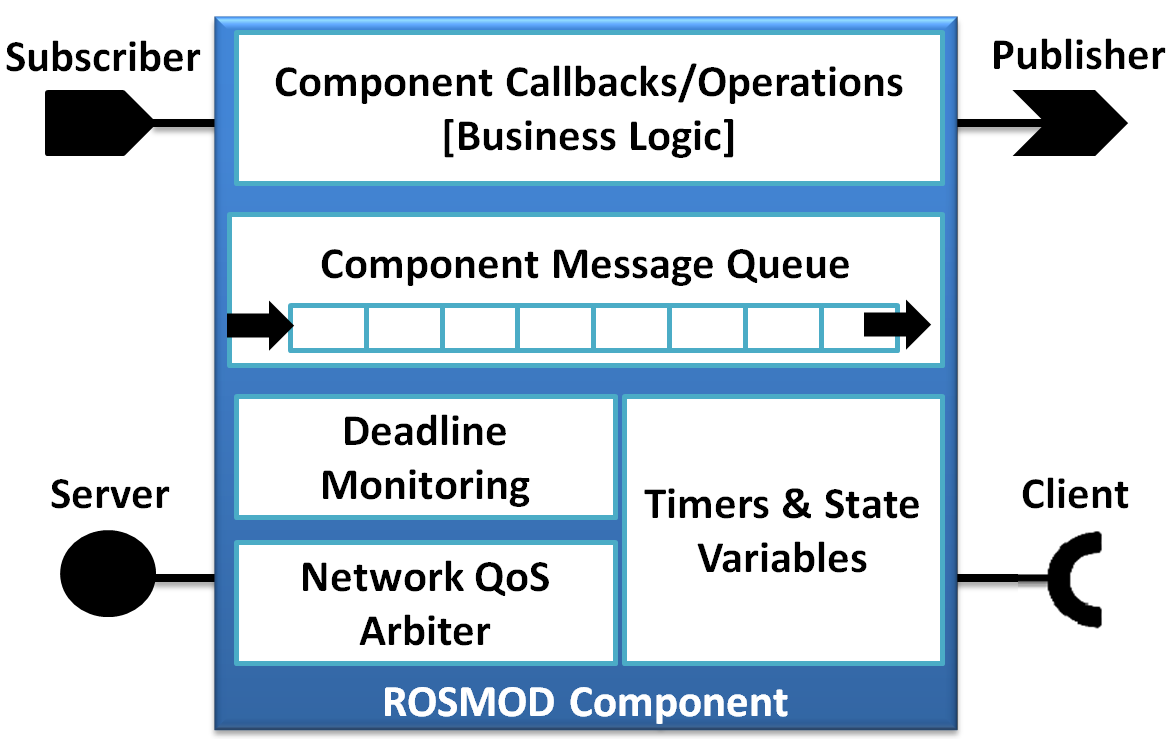
\includegraphics{ROSMOD_Component.png}}

Each component has a single thread called the ``Component Executor Thread''. This thread handles all requests from external entities (other components) and infrastructural triggers (timer expiry). This thread is therefore responsible for executing all triggered callbacks e.g. subscriber callbacks, server callbacks \& timer callbacks. To facilitate interactions with other components, each component also has a ``Component Message Queue''. This queue \emph{holds} requests received from other interacting entities.

The following figure shows a simple Client-Server component interaction. Component A is periodically triggered by a timer. At each timer expiry, Component A makes a blocking remote procedure call to Component B using its client port. This service request, on reaching Component B, is enqueued onto Component B's message queue. When this request reaches the front of the queue, the corresponding server-side callback is executed by the Component B executor thread and the response is returned back to Component A. This message queue based interaction between component entities is also true for timers. When the timer in Component A expires, a timer callback request is enqueued onto its message queue and eventually handled.

{\hfill\scalebox{0.750000}{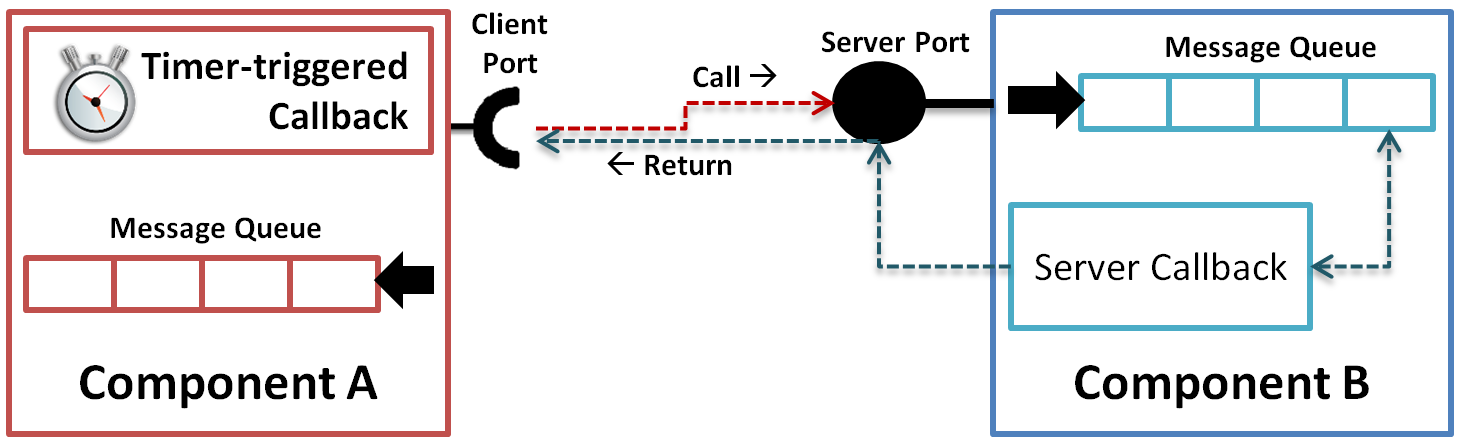
\includegraphics{Component_Message_Queue.png}}\hfill}


\subsubsection{ROSMOD Nodes}
\label{Introduction:rosmod-nodes}
ROSMOD Nodes are deployable processes that run the application/package. These Nodes contain one or more \emph{instances} of ROSMOD Components. Therefore, each ROSMOD node contains one or more component threads, each of which (1) uses component ports to push out queries, (2) uses its message queue to receive external requests, and (3) executes triggered callbacks. ROSMOD Nodes are similar to ROS Nodes but follow a strict structure and behavior.


\section{Modeling Language}
\label{Modeling_Language:modeling-language}\label{Modeling_Language::doc}

\subsection{Software Model}
\label{Modeling_Language:software-model}
The Software model completely describes a ROS Workspace. Every ROS Workspace contains one or more packages. Each package contains \href{http://wiki.ros.org/Messages}{messages}, \href{http://wiki.ros.org/Services}{services} and components.


\subsection{Hardware Model}
\label{Modeling_Language:hardware-model}

\subsection{Deployment Model}
\label{Modeling_Language:deployment-model}

\section{Graphical User Interface}
\label{Editor::doc}\label{Editor:graphical-user-interface}

\section{Code Generators}
\label{Code_Generators:code-generators}\label{Code_Generators::doc}

\section{Deployment Infrastructure}
\label{Deployment_Infrastructure:deployment-infrastructure}\label{Deployment_Infrastructure::doc}

\section{Logging Framework}
\label{Logging_Framework::doc}\label{Logging_Framework:logging-framework}

\section{Tutorial}
\label{Tutorial::doc}\label{Tutorial:tutorial}

\section{Library Reference}
\label{Library_Reference:library-reference}\label{Library_Reference::doc}\label{Library_Reference:id1}

\subsection{Grammar Metaclass}
\label{Library_Reference:grammar-metaclass}

\subsubsection{Grammar\_MetaClass}
\label{class_Grammar_MetaClass:grammar-metaclass}\label{class_Grammar_MetaClass::doc}\phantomsection\label{class_Grammar_MetaClass:id1}\index{Grammar\_MetaClass (built-in class)}

\begin{fulllineitems}
\phantomsection\label{class_Grammar_MetaClass:Grammar_MetaClass}\pysiglinewithargsret{\strong{class }\bfcode{Grammar\_MetaClass}}{\emph{type}}{}
Metaclass for generating on-the-fly ANTLR 4 grammar-specific listener functions to parse model files ( *.rml \textbar{} *.rhw \textbar{} *.rdp )
\index{\_\_new\_\_() (Grammar\_MetaClass method)}

\begin{fulllineitems}
\phantomsection\label{class_Grammar_MetaClass:Grammar_MetaClass.__new__}\pysiglinewithargsret{\bfcode{\_\_new\_\_}}{\emph{name}, \emph{bases}, \emph{attrs}}{}
Intercept ROSMOD Object creation and add attributes to the objects based on model parsing
\begin{quote}\begin{description}
\item[{Parameters}] \leavevmode\begin{itemize}
\item {} 
\textbf{name} -- Name of the to-be-created class

\item {} 
\textbf{bases} -- List of all base classes of the to-be-created class

\item {} 
\textbf{attrs} -- Dictionary of all attributes in the to-be-created class

\end{itemize}

\end{description}\end{quote}

\end{fulllineitems}


\end{fulllineitems}



\subsection{Project Classes}
\label{Library_Reference:project-classes}

\subsubsection{ROSMOD Project}
\label{class_Project::doc}\label{class_Project:rosmod-project}\index{ROSMOD\_Project (built-in class)}

\begin{fulllineitems}
\phantomsection\label{class_Project:ROSMOD_Project}\pysiglinewithargsret{\strong{class }\bfcode{ROSMOD\_Project}}{\emph{Drawable\_Object}}{}
The high-level interface to a ROSMOD Project
\index{\_\_init\_\_() (ROSMOD\_Project method)}

\begin{fulllineitems}
\phantomsection\label{class_Project:ROSMOD_Project.__init__}\pysiglinewithargsret{\bfcode{\_\_init\_\_}}{\emph{**kwargs}}{}
Initialize an empty ROSMOD Project.

\end{fulllineitems}

\index{new() (ROSMOD\_Project method)}

\begin{fulllineitems}
\phantomsection\label{class_Project:ROSMOD_Project.new}\pysiglinewithargsret{\bfcode{new}}{\emph{project\_name}, \emph{project\_path}, \emph{workspace\_name}, \emph{hardware\_name}, \emph{deployment\_name}\optional{, \emph{q=None}}}{}
Create a new ROSMOD Project.
\begin{quote}\begin{description}
\item[{Parameters}] \leavevmode\begin{itemize}
\item {} 
\textbf{project\_name} (\href{http://docs.python.org/library/functions.html\#str}{\emph{str}}) -- The name of the ROSMOD Project

\item {} 
\textbf{project\_path} (\href{http://docs.python.org/library/functions.html\#str}{\emph{str}}) -- The absolute path to the root directory of the ROSMOD Project

\item {} 
\textbf{workspace\_name} (\href{http://docs.python.org/library/functions.html\#str}{\emph{str}}) -- The name of the ROSMOD Software Model and the generated ROS Workspace

\item {} 
\textbf{hardware\_name} (\href{http://docs.python.org/library/functions.html\#str}{\emph{str}}) -- The name of the ROSMOD Hardware Model

\item {} 
\textbf{deployment\_name} (\href{http://docs.python.org/library/functions.html\#str}{\emph{str}}) -- The name of the ROSMOD Deployment Model

\end{itemize}

\end{description}\end{quote}

\end{fulllineitems}

\index{open() (ROSMOD\_Project method)}

\begin{fulllineitems}
\phantomsection\label{class_Project:ROSMOD_Project.open}\pysiglinewithargsret{\bfcode{open}}{\emph{project\_path}\optional{, \emph{progressQ = None}}}{}
Open an existing ROSMOD Project
\begin{quote}\begin{description}
\item[{Parameters}] \leavevmode
\textbf{project\_Path} (\href{http://docs.python.org/library/functions.html\#str}{\emph{str}}) -- The absolute path to the root directory of the ROSMOD Project

\end{description}\end{quote}

\end{fulllineitems}

\index{parse\_msg() (ROSMOD\_Project method)}

\begin{fulllineitems}
\phantomsection\label{class_Project:ROSMOD_Project.parse_msg}\pysiglinewithargsret{\bfcode{parse\_msg}}{\emph{dirname}}{}
Parse all msg (message) files in the Software Model
\begin{quote}\begin{description}
\item[{Parameters}] \leavevmode
\textbf{dirname} (\href{http://docs.python.org/library/functions.html\#str}{\emph{str}}) -- The path to the msg directory in the ROSMOD Software Model

\end{description}\end{quote}

\end{fulllineitems}

\index{parse\_srv() (ROSMOD\_Project method)}

\begin{fulllineitems}
\phantomsection\label{class_Project:ROSMOD_Project.parse_srv}\pysiglinewithargsret{\bfcode{parse\_srv}}{\emph{dirname}}{}
Parse all srv (service) files in the Software Model
\begin{quote}\begin{description}
\item[{Parameters}] \leavevmode
\textbf{dirname} (\href{http://docs.python.org/library/functions.html\#str}{\emph{str}}) -- The path to the srv directory in the ROSMOD Software Model

\end{description}\end{quote}

\end{fulllineitems}

\index{parse\_abl() (ROSMOD\_Project method)}

\begin{fulllineitems}
\phantomsection\label{class_Project:ROSMOD_Project.parse_abl}\pysiglinewithargsret{\bfcode{parse\_abl}}{\emph{dirname}}{}
Parse all abl (abstract business logic) files in the Software Model
\begin{quote}\begin{description}
\item[{Parameters}] \leavevmode
\textbf{dirname} (\href{http://docs.python.org/library/functions.html\#str}{\emph{str}}) -- The path to the abl directory in the ROSMOD Software Model

\end{description}\end{quote}

\end{fulllineitems}

\index{parse\_pnp() (ROSMOD\_Project method)}

\begin{fulllineitems}
\phantomsection\label{class_Project:ROSMOD_Project.parse_pnp}\pysiglinewithargsret{\bfcode{parse\_pnp}}{\emph{dirname}}{}
Parse all pnp (port network profiles) files in the Software Model
\begin{quote}\begin{description}
\item[{Parameters}] \leavevmode
\textbf{dirname} (\href{http://docs.python.org/library/functions.html\#str}{\emph{str}}) -- The path to the pnp directory in the ROSMOD Software Model

\end{description}\end{quote}

\end{fulllineitems}

\index{parse\_snp() (ROSMOD\_Project method)}

\begin{fulllineitems}
\phantomsection\label{class_Project:ROSMOD_Project.parse_snp}\pysiglinewithargsret{\bfcode{parse\_snp}}{\emph{dirname}}{}
Parse all snp (system network profiles) files in the Hardware Model
\begin{quote}\begin{description}
\item[{Parameters}] \leavevmode
\textbf{dirname} (\href{http://docs.python.org/library/functions.html\#str}{\emph{str}}) -- The path to the snp directory in the ROSMOD Hardware Model

\end{description}\end{quote}

\end{fulllineitems}

\index{parse\_rml() (ROSMOD\_Project method)}

\begin{fulllineitems}
\phantomsection\label{class_Project:ROSMOD_Project.parse_rml}\pysiglinewithargsret{\bfcode{parse\_rml}}{\emph{filename}}{}
Parse the provided rml file (ROSMOD Software Model)
\begin{quote}\begin{description}
\item[{Parameters}] \leavevmode
\textbf{filename} (\href{http://docs.python.org/library/functions.html\#str}{\emph{str}}) -- The name of the .rml file

\end{description}\end{quote}

\end{fulllineitems}

\index{parse\_rhw() (ROSMOD\_Project method)}

\begin{fulllineitems}
\phantomsection\label{class_Project:ROSMOD_Project.parse_rhw}\pysiglinewithargsret{\bfcode{parse\_rhw}}{\emph{filename}}{}
Parse the provided rhw file (ROSMOD Hardware Model)
\begin{quote}\begin{description}
\item[{Parameters}] \leavevmode
\textbf{filename} (\href{http://docs.python.org/library/functions.html\#str}{\emph{str}}) -- The name of the .rhw file

\end{description}\end{quote}

\end{fulllineitems}

\index{parse\_rdp() (ROSMOD\_Project method)}

\begin{fulllineitems}
\phantomsection\label{class_Project:ROSMOD_Project.parse_rdp}\pysiglinewithargsret{\bfcode{parse\_rdp}}{\emph{filename}}{}
Parse the provided rdp file (ROSMOD Deployment Model)
\begin{quote}\begin{description}
\item[{Parameters}] \leavevmode
\textbf{filename} (\href{http://docs.python.org/library/functions.html\#str}{\emph{str}}) -- The name of the .rdp file

\end{description}\end{quote}

\end{fulllineitems}

\index{parse\_models() (ROSMOD\_Project method)}

\begin{fulllineitems}
\phantomsection\label{class_Project:ROSMOD_Project.parse_models}\pysiglinewithargsret{\bfcode{parse\_models}}{\optional{\emph{progressQ=None}}}{}
Parse all Software, Hardware and Deployment models in the ROSMOD Project

\end{fulllineitems}

\index{check\_workspace() (ROSMOD\_Project method)}

\begin{fulllineitems}
\phantomsection\label{class_Project:ROSMOD_Project.check_workspace}\pysiglinewithargsret{\bfcode{check\_workspace}}{}{}
Check for an existing ROS Workspace in the ROSMOD Project in order to preserve any code between code-preservation markers

\end{fulllineitems}

\index{generate\_workspace() (ROSMOD\_Project method)}

\begin{fulllineitems}
\phantomsection\label{class_Project:ROSMOD_Project.generate_workspace}\pysiglinewithargsret{\bfcode{generate\_workspace}}{}{}
Generate a ROS Workspace from the Software Model. The workspace is generated at PROJECT\_ROOT/01-Software/\textless{}workspace\_name\textgreater{}

\end{fulllineitems}

\index{generate\_xml() (ROSMOD\_Project method)}

\begin{fulllineitems}
\phantomsection\label{class_Project:ROSMOD_Project.generate_xml}\pysiglinewithargsret{\bfcode{generate\_xml}}{}{}
Generate Deployment XML files for all ROS nodes in the Deployment Model

\end{fulllineitems}

\index{generate\_cpn() (ROSMOD\_Project method)}

\begin{fulllineitems}
\phantomsection\label{class_Project:ROSMOD_Project.generate_cpn}\pysiglinewithargsret{\bfcode{generate\_cpn}}{}{}
Generate a Colored Petri Net timing analysis model for the ROSMOD Project

\end{fulllineitems}

\index{resolve\_references() (ROSMOD\_Project method)}

\begin{fulllineitems}
\phantomsection\label{class_Project:ROSMOD_Project.resolve_references}\pysiglinewithargsret{\bfcode{resolve\_references}}{\optional{\emph{progressQ = None}}}{}
Resolve all missing object references after parsing models

\end{fulllineitems}

\index{save\_rml() (ROSMOD\_Project method)}

\begin{fulllineitems}
\phantomsection\label{class_Project:ROSMOD_Project.save_rml}\pysiglinewithargsret{\bfcode{save\_rml}}{\optional{\emph{path=''``}}}{}
Save a modified workspace (.rml) file
\begin{quote}\begin{description}
\item[{Parameters}] \leavevmode
\textbf{path} (\href{http://docs.python.org/library/functions.html\#str}{\emph{str}}) -- Optional path where the .rml file will be saved

\end{description}\end{quote}

\end{fulllineitems}

\index{save\_rhw() (ROSMOD\_Project method)}

\begin{fulllineitems}
\phantomsection\label{class_Project:ROSMOD_Project.save_rhw}\pysiglinewithargsret{\bfcode{save\_rhw}}{\optional{\emph{path=''``}}}{}
Save a modified workspace (.rhw) file
\begin{quote}\begin{description}
\item[{Parameters}] \leavevmode
\textbf{path} (\href{http://docs.python.org/library/functions.html\#str}{\emph{str}}) -- Optional path where the .rhw file will be saved

\end{description}\end{quote}

\end{fulllineitems}

\index{save\_rdp() (ROSMOD\_Project method)}

\begin{fulllineitems}
\phantomsection\label{class_Project:ROSMOD_Project.save_rdp}\pysiglinewithargsret{\bfcode{save\_rdp}}{\optional{\emph{path=''``}}}{}
Save a modified workspace (.rdp) file
\begin{quote}\begin{description}
\item[{Parameters}] \leavevmode
\textbf{path} (\href{http://docs.python.org/library/functions.html\#str}{\emph{str}}) -- Optional path where the .rdp file will be saved

\end{description}\end{quote}

\end{fulllineitems}

\index{save\_msg() (ROSMOD\_Project method)}

\begin{fulllineitems}
\phantomsection\label{class_Project:ROSMOD_Project.save_msg}\pysiglinewithargsret{\bfcode{save\_msg}}{\emph{msg\_object}}{}
Save a modified msg object to file
\begin{quote}\begin{description}
\item[{Parameters}] \leavevmode
\textbf{msg\_object} -- Message Object to be saved

\end{description}\end{quote}

\end{fulllineitems}

\index{save\_srv() (ROSMOD\_Project method)}

\begin{fulllineitems}
\phantomsection\label{class_Project:ROSMOD_Project.save_srv}\pysiglinewithargsret{\bfcode{save\_srv}}{\emph{srv\_object}}{}
Save a modified srv object to file
\begin{quote}\begin{description}
\item[{Parameters}] \leavevmode
\textbf{srv\_object} -- Service Object to be saved

\end{description}\end{quote}

\end{fulllineitems}

\index{save\_abl() (ROSMOD\_Project method)}

\begin{fulllineitems}
\phantomsection\label{class_Project:ROSMOD_Project.save_abl}\pysiglinewithargsret{\bfcode{save\_abl}}{\emph{port\_object}}{}
Save a modified abstract business logic to file
\begin{quote}\begin{description}
\item[{Parameters}] \leavevmode
\textbf{port\_object} -- Port Object that contains an abstract business logic

\end{description}\end{quote}

\end{fulllineitems}

\index{save\_pnp() (ROSMOD\_Project method)}

\begin{fulllineitems}
\phantomsection\label{class_Project:ROSMOD_Project.save_pnp}\pysiglinewithargsret{\bfcode{save\_pnp}}{\emph{port\_object}}{}
Save a modified port network profile to file
\begin{quote}\begin{description}
\item[{Parameters}] \leavevmode
\textbf{port\_object} -- Port Object that contains a port network profile

\end{description}\end{quote}

\end{fulllineitems}

\index{save\_snp() (ROSMOD\_Project method)}

\begin{fulllineitems}
\phantomsection\label{class_Project:ROSMOD_Project.save_snp}\pysiglinewithargsret{\bfcode{save\_snp}}{\emph{port\_object}}{}
Save a modified system network profile to file
\begin{quote}\begin{description}
\item[{Parameters}] \leavevmode
\textbf{port\_object} -- Port Object that contains a system network profile

\end{description}\end{quote}

\end{fulllineitems}

\index{save() (ROSMOD\_Project method)}

\begin{fulllineitems}
\phantomsection\label{class_Project:ROSMOD_Project.save}\pysiglinewithargsret{\bfcode{save}}{\optional{\emph{project\_name=''``}}\optional{, \emph{project\_path=''``}}}{}
Used to ``Save'' or ``Save-As'' an entire ROSMOD Project
\begin{quote}\begin{description}
\item[{Parameters}] \leavevmode\begin{itemize}
\item {} 
\textbf{project\_name} (\href{http://docs.python.org/library/functions.html\#str}{\emph{str}}) -- Name of ROSMOD Project used for Save-As

\item {} 
\textbf{project\_path} (\href{http://docs.python.org/library/functions.html\#str}{\emph{str}}) -- Absolute path to ROSMOD Project used for Save-As

\end{itemize}

\end{description}\end{quote}

\end{fulllineitems}


\end{fulllineitems}



\subsubsection{ROSMOD\_Generator}
\label{class_Generator:rosmod-generator}\label{class_Generator::doc}\index{ROSMOD\_Generator (built-in class)}

\begin{fulllineitems}
\phantomsection\label{class_Generator:ROSMOD_Generator}\pysigline{\strong{class }\bfcode{ROSMOD\_Generator}}
Primary Generator class for ROSMOD
\index{generate\_workspace() (ROSMOD\_Generator method)}

\begin{fulllineitems}
\phantomsection\label{class_Generator:ROSMOD_Generator.generate_workspace}\pysiglinewithargsret{\bfcode{generate\_workspace}}{\emph{workspace}, \emph{path}}{}
Generate the ROS Workspace and build system from the Software Model
\begin{quote}\begin{description}
\item[{Parameters}] \leavevmode\begin{itemize}
\item {} 
\textbf{workspace} -- The ROS\_Workspace object to traverse

\item {} 
\textbf{path} (\href{http://docs.python.org/library/functions.html\#str}{\emph{str}}) -- The absolute path to the to-be-generated workspace directory

\end{itemize}

\end{description}\end{quote}

\end{fulllineitems}

\index{generate\_xml() (ROSMOD\_Generator method)}

\begin{fulllineitems}
\phantomsection\label{class_Generator:ROSMOD_Generator.generate_xml}\pysiglinewithargsret{\bfcode{generate\_xml}}{\emph{deployments}, \emph{deployment\_path}}{}
Generate Deployment-specific ROS Node XML files from the Deployment Model
\begin{quote}\begin{description}
\item[{Parameters}] \leavevmode\begin{itemize}
\item {} 
\textbf{deployments} -- The list of all ROS\_Deployment objects in 03-Deployment directory

\item {} 
\textbf{deployment\_path} -- The absolute path to the Deployment directory

\end{itemize}

\end{description}\end{quote}

\end{fulllineitems}

\index{generate\_cpn() (ROSMOD\_Generator method)}

\begin{fulllineitems}
\phantomsection\label{class_Generator:ROSMOD_Generator.generate_cpn}\pysiglinewithargsret{\bfcode{generate\_cpn}}{\emph{workspace}, \emph{deployments}, \emph{deployment\_path}}{}
Generate a Colored Petri Net-based Timing Analysis Model for the Project
\begin{quote}\begin{description}
\item[{Parameters}] \leavevmode\begin{itemize}
\item {} 
\textbf{workspace} -- The ROS\_Workspace object to traverse

\item {} 
\textbf{deployments} -- The list of all ROS\_Deployment objects in 03-Deployment directory

\item {} 
\textbf{deployment\_path} -- The absolute path to the Deployment directory

\end{itemize}

\end{description}\end{quote}

\end{fulllineitems}


\end{fulllineitems}



\subsubsection{ROSMOD\_Loader}
\label{class_Loader::doc}\label{class_Loader:rosmod-loader}\index{ROSMOD\_Loader (built-in class)}

\begin{fulllineitems}
\phantomsection\label{class_Loader:ROSMOD_Loader}\pysigline{\strong{class }\bfcode{ROSMOD\_Loader}}
Loads an existing ROS Workspace for Code Preservation
\index{load() (ROSMOD\_Loader method)}

\begin{fulllineitems}
\phantomsection\label{class_Loader:ROSMOD_Loader.load}\pysiglinewithargsret{\bfcode{load}}{\emph{workspace}, \emph{path}}{}
Load an existing ROS workspace and preserve code blocks between code-preservation markers so that regeneration does not completely overwrite existing work
\begin{quote}\begin{description}
\item[{Parameters}] \leavevmode\begin{itemize}
\item {} 
\textbf{workspace} -- The ROS\_Workspace object to traverse

\item {} 
\textbf{path} (\href{http://docs.python.org/library/functions.html\#str}{\emph{str}}) -- The absolute path to the ROS workspace directory

\end{itemize}

\end{description}\end{quote}

\end{fulllineitems}


\end{fulllineitems}



\subsubsection{ROSMOD\_Software\_Builder}
\label{class_Software_Builder::doc}\label{class_Software_Builder:rosmod-software-builder}\index{ROSMOD\_Software\_Builder (built-in class)}

\begin{fulllineitems}
\phantomsection\label{class_Software_Builder:ROSMOD_Software_Builder}\pysiglinewithargsret{\strong{class }\bfcode{ROSMOD\_Software\_Builder}}{\emph{ROSMOD\_SoftwareListener}}{}
Builds a Software Object Tree from parsing the .rml file in 01-Software/*
\begin{quote}\begin{description}
\item[{Variables}] \leavevmode
\href{http://docs.python.org/reference/datamodel.html\#\_\_metaclass\_\_}{\textbf{\_\_metaclass\_\_}} -- {\hyperref[class_Grammar_MetaClass:id1]{\emph{Grammar\_MetaClass}}}

\end{description}\end{quote}
\index{\_\_init\_\_() (ROSMOD\_Software\_Builder method)}

\begin{fulllineitems}
\phantomsection\label{class_Software_Builder:ROSMOD_Software_Builder.__init__}\pysiglinewithargsret{\bfcode{\_\_init\_\_}}{\emph{project}}{}
Initialize the root of the Software Object Tree, a ``ROS\_RML'' class object
\begin{quote}\begin{description}
\item[{Parameters}] \leavevmode
\textbf{project} -- The ROSMOD\_Project object that is the parent of the Software model

\end{description}\end{quote}

\end{fulllineitems}


\end{fulllineitems}



\subsubsection{ROSMOD\_Hardware\_Builder}
\label{class_Hardware_Builder:rosmod-hardware-builder}\label{class_Hardware_Builder::doc}\index{ROSMOD\_Hardware\_Builder (built-in class)}

\begin{fulllineitems}
\phantomsection\label{class_Hardware_Builder:ROSMOD_Hardware_Builder}\pysigline{\strong{class }\bfcode{ROSMOD\_Hardware\_Builder}}
Builds a Hardware Object Tree from parsing the .rhw files in 02-Hardware/*
\begin{quote}\begin{description}
\item[{Variables}] \leavevmode
\href{http://docs.python.org/reference/datamodel.html\#\_\_metaclass\_\_}{\textbf{\_\_metaclass\_\_}} -- {\hyperref[class_Grammar_MetaClass:id1]{\emph{Grammar\_MetaClass}}}

\end{description}\end{quote}
\index{\_\_init\_\_() (ROSMOD\_Hardware\_Builder method)}

\begin{fulllineitems}
\phantomsection\label{class_Hardware_Builder:ROSMOD_Hardware_Builder.__init__}\pysiglinewithargsret{\bfcode{\_\_init\_\_}}{\emph{project}}{}
Initialize the root of the Hardware Object Tree, a ``ROS\_RHW'' class object
\begin{quote}\begin{description}
\item[{Parameters}] \leavevmode
\textbf{project} -- The ROSMOD\_Project object that is the parent of the Software model

\end{description}\end{quote}

\end{fulllineitems}


\end{fulllineitems}



\subsubsection{ROSMOD\_Deployment\_Builder}
\label{class_Deployment_Builder::doc}\label{class_Deployment_Builder:rosmod-deployment-builder}\index{ROSMOD\_Deployment\_Builder (built-in class)}

\begin{fulllineitems}
\phantomsection\label{class_Deployment_Builder:ROSMOD_Deployment_Builder}\pysigline{\strong{class }\bfcode{ROSMOD\_Deployment\_Builder}}
Builds a Deployment Object Tree from parsing the .rdp files in 03-Deployment/
\begin{quote}\begin{description}
\item[{Variables}] \leavevmode
\href{http://docs.python.org/reference/datamodel.html\#\_\_metaclass\_\_}{\textbf{\_\_metaclass\_\_}} -- {\hyperref[class_Grammar_MetaClass:id1]{\emph{Grammar\_MetaClass}}}

\end{description}\end{quote}
\index{\_\_init\_\_() (ROSMOD\_Deployment\_Builder method)}

\begin{fulllineitems}
\phantomsection\label{class_Deployment_Builder:ROSMOD_Deployment_Builder.__init__}\pysiglinewithargsret{\bfcode{\_\_init\_\_}}{\emph{project}}{}
Initialize the root of the Deployment Object Tree, a ``ROS\_RDP'' class object
\begin{quote}\begin{description}
\item[{Parameters}] \leavevmode
\textbf{project} -- The ROSMOD\_Project object that is the parent of the Software model

\end{description}\end{quote}

\end{fulllineitems}


\end{fulllineitems}



\chapter{Indices and tables}
\label{index:indices-and-tables}\begin{itemize}
\item {} 
\emph{genindex}

\item {} 
\emph{modindex}

\item {} 
\emph{search}

\end{itemize}



\renewcommand{\indexname}{Index}
\printindex
\end{document}
